\documentclass[a4j,dvipdfmx]{jsarticle}
\usepackage{graphicx}
%\usepackage{multirow}
%\usepackage{color}
%\usepackage{lscape}
%\usepackage{ascmac}
%\usepackage{txfonts}


\usepackage{listings, jlisting}
\renewcommand{\lstlistingname}{リスト}
\lstset{
  language={C},
  basicstyle=\ttfamily\scriptsize,
  commentstyle=\textit,
  classoffset=1,
  keywordstyle=\bfseries,
  frame=tRBl,
  framesep=5pt,
  showstringspaces=true,
  numbers=left,
  stepnumber=1,
  numberstyle=\tiny,
  tabsize=2
}


%% %subsubsubsectionの定義(できるだけ使わない方向で)
%% \makeatletter
%% \newcommand{\subsubsubsection}{\@startsection{paragraph}{4}{\z@}%
%%   {1.0\Cvs \@plus.5\Cdp \@minus.2\Cdp}%
%%   {.1\Cvs \@plus.3\Cdp}%
%%   {\reset@font\sffamily\normalsize}
%% }
%% \makeatother
%% \setcounter{secnumdepth}{4}
%ここまでsubsubsubsectionの定義

\begin{document}

\title{計算機科学実験及び演習4\\コンピュータグラフィックス\\発展課題}
\author{工学部情報学科3回生 1029255242\\勝見久央}
\date{作成日: \today} % コンパイル時の日付が自動で挿入される
\maketitle
%文字コードはUTF-8推奨.それ以外ではline2のcontentsline~にエラー発生.
%選択範囲コメントアウトは選択中にM-;
%%%%%%%%%%%%%%%%%%%%%%%%%%%%%%%%%%%%%%%%%%%%%%%%%%%%%%%%%%%%%%%%%%%%%%
%ソースコードの貼付け
%% \lstinputlisting[caption=キャプション,label=ラベル,breaklines=true]
%% {./kadai01.sc}
%%次でも可
%% \begin{lstlisting}
%% \end{lstlisting}
\section{概要}
本レポートは必須課題1〜3を終了後に取り組んだ発展課題と、
その内容についての概要を記したレポートである.

%% ============================================================================================
\section{課題4}
本課題ではグーローシェーディングのみを実装した.
\subsection{プログラム本体}
プログラム本体は次のようになった.
\lstinputlisting[caption=kadai04.c,label=kadai04.c,breaklines=true]{./kadai04.c}
\section{実行例}
kadai04.cと同一のディレクトリに次のプログラムを置き、
\lstinputlisting[caption=EvalKadai04.sh,label=EvalKadai04.sh,breaklines=true]{./EvalKadai04.sh}
さらに同一ディレクトリ内のディレクトリsampleの中に対象とするVRMLファイルを置いて、
\begin{lstlisting}
$ sh EvalKadai04.sh
\end{lstlisting}
を実行した.
出力画像は図\ref{fig:k4-av5}のようになった.
\begin{figure}[hp]
  \begin{center}
    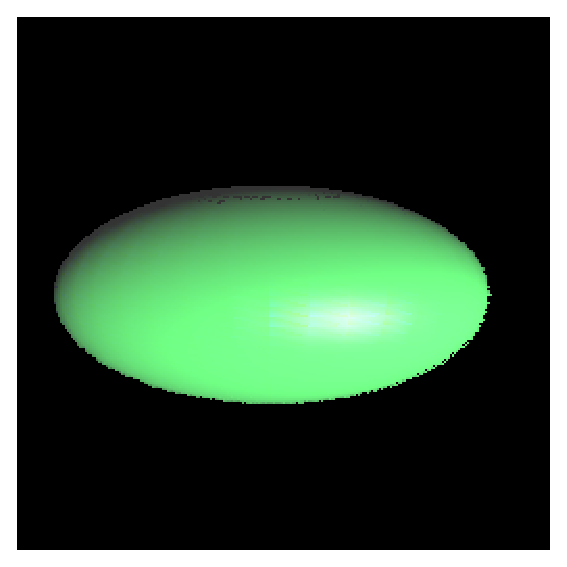
\includegraphics[clip,scale=0.5]{images/Kadai04ForAv5.eps}
    \caption{av5.wrlの出力結果}
    \label{fig:k4-av5}
  \end{center}
\end{figure}

%% ============================================================================================
\section{課題5}
本課題ではまず環境マッピングをフォーンシェーディングによって
実装した.さらに課題4では実装しなかったカメラ位置の変更機能をプログラムに加えた.
なお、便宜上、カメラ位置についてはコマンドライン変数よりx座標のみを指定する仕様としている.
\section{実行例}
kadai05.cと同一のディレクトリに次のプログラムを置き、
\lstinputlisting[caption=EvalKadai05.sh,label=EvalKadai05.sh,breaklines=true]{./EvalKadai05.sh}
さらに同一ディレクトリ内のディレクトリsampleの中に対象とするVRMLファイルを置いて、
\begin{lstlisting}
$ sh EvalKadai05.sh
\end{lstlisting}
を実行した.
出力画像は図\ref{fig:k5-0}、図\ref{fig:k5-1}、図\ref{fig:k5-2}のようになった.
\begin{figure}[hp]
  \begin{center}
    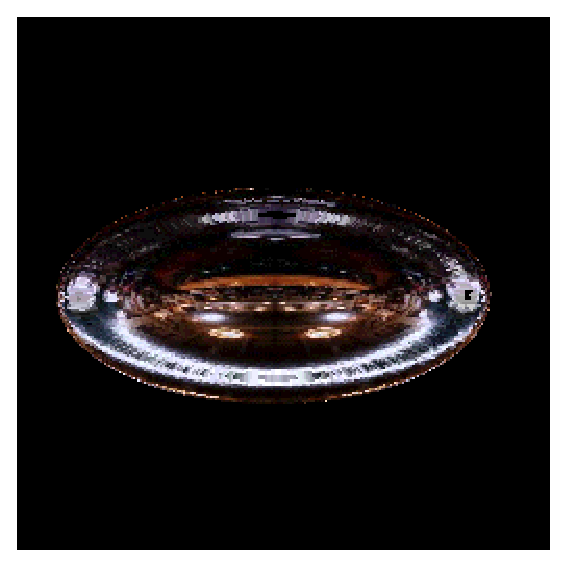
\includegraphics[clip,scale=0.5]{images/Kadai05ForAv5-0.eps}
    \caption{カメラのx座標が0.0の時のav5の出力結果}
    \label{fig:k5-0}
  \end{center}
\end{figure}
\begin{figure}[hp]
  \begin{center}
    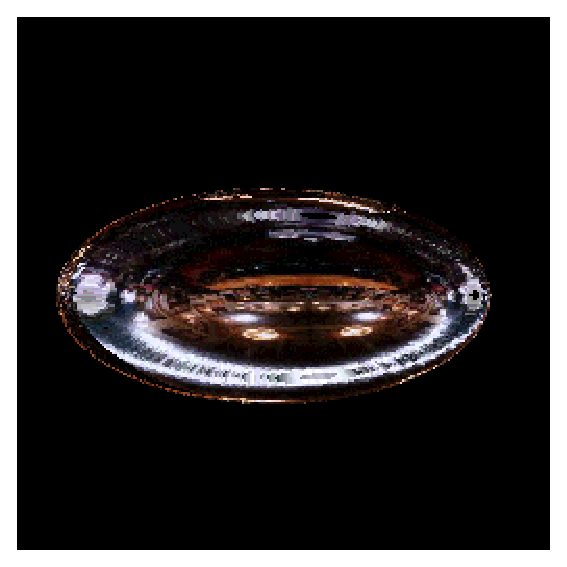
\includegraphics[clip,scale=0.5]{images/Kadai05ForAv5-1.eps}
    \caption{カメラのx座標が50.0の時のav5の出力結果}
    \label{fig:k5-1}
  \end{center}
\end{figure}
\begin{figure}[hp]
  \begin{center}
    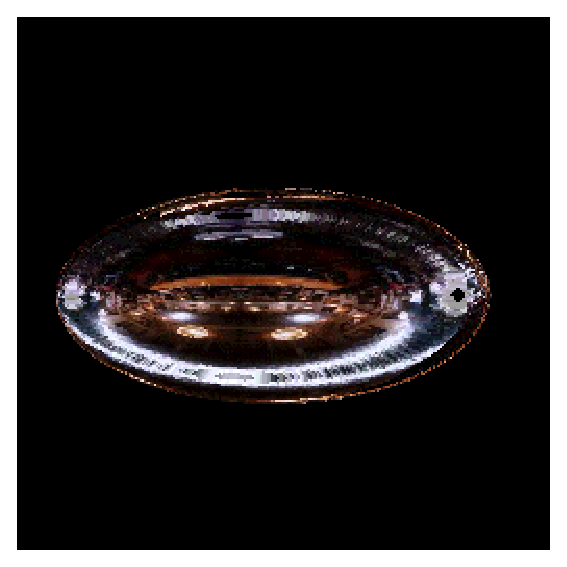
\includegraphics[clip,scale=0.5]{images/Kadai05ForAv5-2.eps}
    \caption{カメラのx座標が-50.0の時のav5の出力結果}
    \label{fig:k5-2}
  \end{center}
\end{figure}

\end{document}
